%! Author = vsharma
%! Date = 25.09.2022
% !TeX spellcheck = en_EN

\chapter{Problem Statement}

\par Due to the increase in the rate of cybercrime attempts, growing amounts of data, digital business models, insider threats, human error, etc., security remains a very important topic for companies and their customers \cite{40}.
 These crimes basically refer to the misuse of information and technology for illegal and unauthorized access to resources as seen in figure \ref{fig:securityAttack}.
 Despite the development of offensive tools and
capabilities, the number of security attacks has not been
fully addressed on a truly global \cite{50}.
 Based on the different research work and literature, this chapter highlights various security vulnerabilities in different AWS services.

\begin{figure}
    \centering
    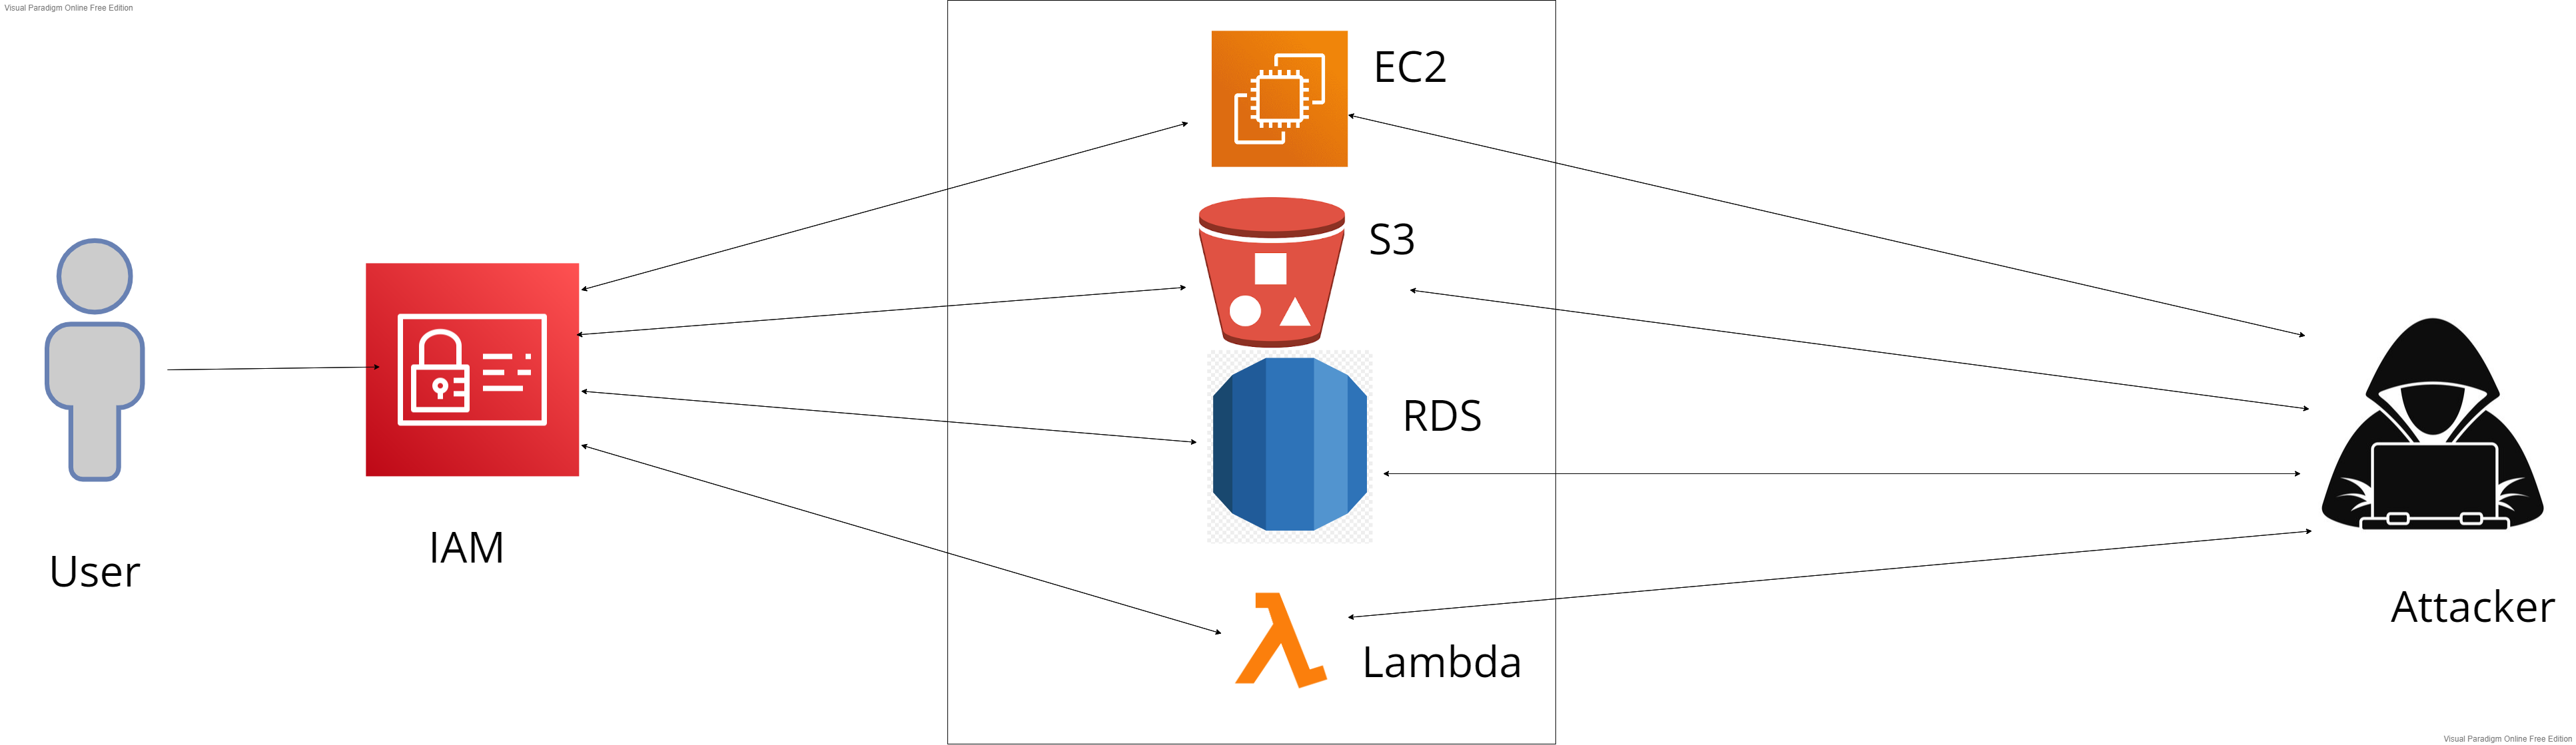
\includegraphics[width=\textwidth]{securityAttack.png}
    \caption{AWS Services Security vulnerabilities}
    \label{fig:securityAttack}
\end{figure}

\section{Identification of Security Vulnerabilities}

\par This section lists the several security vulnerabilities and misconfigurations identified in five AWS services
based on literature, the \gls{owasp} vulnerability list
\cite{51},
\gls{cisa}
\cite{52}, \gls{idc} \cite{53}.


\begin{itemize}
    \item \textbf{Excessive privileges:} Additional Permissive Policies granted to the users beyond what they need.
    This type
    of security vulnerability occurs when the users are
    granted more access than required for their job
    \cite{54}. It is
    sometimes hard to keep up with every user’s permission as every application and system has its own application
    model \cite{55}.
\end{itemize}

\begin{itemize}
    \item \textbf{Insider threat:} Insider threat refers to a person who has the required access rights to an
    information system and misuses his privileges.
    In the last years, it has been experienced that most companies have outsourced their IT infrastructure.
    Outsourcing affects the organization’s risk profile inevitably.
    Characterization of such attackers is not straightforward.
    For example, consider an employee who has been fired.
    In order to take revenge on his former employer, the
    employee plans an attack.
    Even though the employee's access rights should have been revoked, and the employee is not considered a
    legitimate user anymore, if the employee still has
    access to the infrastructure using a backdoor the employee has previously installed, this employee is still considered an insider threat \cite{56}.

    Insider threats can be classified into two contexts:
    \begin{itemize}
        \item \textbf{Cloud provider:} Where the insider
        is an employee working for the cloud provider i.e
        ., a cloud provider has a malicious system
        administrator working for them.
        The insider can use the authorized access
        rights to access sensitive information \cite{56}.
    \end{itemize}
    \begin{itemize}
        \item \textbf{Cloud outsourced:} The insider is an employee of an organization, which has outsourced its
        infrastructure to the cloud \cite{56}.
    \end{itemize}
\end{itemize}

\begin{itemize}
    \item \textbf{Misconfiguration:} Management of configuration is the most important part of network management.
    Bad or Incorrect configuration can have dramatic effects on the security and safety of users, applications, and the overall system. Most data breaches and cyber-attacks in cloud infrastructure are due to misconfiguration vulnerabilities and human errors \cite{44}.

    Various misconfiguration vulnerabilities exist in cloud environments.
    A few examples of misconfiguration are: Not
    using MFA, reusing passwords, using the Root account’s access keys, weaker password policy, misconfiguration of S3
    buckets,  misconfiguration of RDS
    instances, etc \cite{55}.
\end{itemize}

\begin{itemize}
    \item \textbf{Instances created from Malicious AMI:} With the organizations moving their infrastructure, data,
    and workload to the cloud, it is important that the
    \gls{ami}
    from the AWS Marketplace that are
    used in creating the EC2 instance are safe. AMI is used to create virtual servers on the AWS environment.
    Malicious AMI pose significant risks as the embedded code can include ransomware, crypto miners, malware, and so
    on {57}.

    An AMI basically includes the following:
    \begin{itemize}
        \item A template (typically an operating system, e.g., Amazon Linux, Ubuntu, etc., an application server and applications) for the root volume of the instance.
    \end{itemize}
    \begin{itemize}
        \item Launch permissions ensuring the authorized accounts can use the AMI to launch instances.
    \end{itemize}
    An instance was investigated by Summit Route in 2018
    where a Monero miner malware was embedded in an
    Ubuntu AMI \cite{57}.
    Similarly, in 2020, researchers at Mitiga during the assessment of an organization’s AWS environment found an
    active crypto miner on an EC2 instance, later during the review, it was revealed that the crypto miner was
    embedded in the AMI used by the organization \cite{58}.
\end{itemize}

\begin{itemize}
    \item \textbf{User data public exposure:} Exposure of user data is a critical vulnerability in cloud environments.
    Instance user data is a metadata field allowing custom code to run after the instance is launched.
    This metadata
    contains code that is exposed to any entity which has access to EC2, even the most basic access to EC2 for
    example, read-only configurations \cite{48}.

    While user data is an efficient way to automate the launch of scripts at instance launch, EC2 user data is a
    significant place where secrets can be unnecessarily exposed.
    For example, if password need to be used as part of
    a script, the user might be tempted to store it as
    plaintext in the script that we input to the user data.
    If the secrets are stored as plain text, then any user with ec2:DescribeInstanceAttribute permission will be able to view the secrets \cite{59}.

    Another example is when an instance pulls an application from a private Git repository.
    As the repository is
    private it can be accessed using the SSH key.
    Often this key is hard coded in the user data.
    Attacker can get
    access to the private source code of the application if the attacker gets access to the instance user data.
    The attacker can access the user data if he is able
    to query the IMDS from the EC2 instance, e.g. using an SSRF
    vulnerability.
    The attacker can read the user data directly from the
    AWS \gls{api} ,if the attacker has valid AWS
    credentials with the ec2:DescribeInstanceAttribute
    IAM permission \cite{60}.
\end{itemize}

\begin{itemize}
    \item \textbf{\gls{ssrf}:} \gls{ssrf} is a web security
    vulnerability allowing an attacker to make requests to an unintended location through the server-side application.

    SSRF tricks the web application to make an HTTP request on behalf of the attacker to a URL. This allows the
    attacker to get access to sensitive data or information that are exposed directly, or the attacker does not have
    access to, for example, AWS metadata, external web services, or other web applications based within the
    organization’s infrastructure.
    Sometimes is it also possible for the attacker to perform arbitrary command
    execution \cite{61}.
    SSRF is mostly encountered \cite{62}:
    \begin{itemize}
        \item If an attribute enables file generation methodology for example PDF generation.
    \end{itemize}
    \begin{itemize}
        \item If there is a file upload such as uploading the scanned images, documents, files, etc.
    \end{itemize}
\end{itemize}

\begin{itemize}
    \item \textbf{Denial of Wallet:} The Denial of Wallet is a form of security vulnerability unique to serverless
    computing,
    that results in financial exhaustion of the victim in the form of inflated usage bills.
    The execution costs are
    primarily increased via excessive function run time, additional resource consumption, and invocation count.
    This
    is usually achieved by exploiting the massive capability for scaling.
    The platform will be capable of handling
    such increased load but will incur costs for doing so
    \cite{63} \cite{64} \cite{65}.
\end{itemize}

\begin{itemize}
    \item \textbf{Public RDS Database instance:} Amazon RDS, a web service that enables setting up and scaling
    relational databases in the cloud for the web applications.
    Minimizing data loss and security risks can be
    ensured by checking the database’s instance for
    restricting unauthorized access and public
    accessibility \cite{66}.

    The RDS instance is within a \gls{vpc}.
    The default VPC consists of three subnets used to 
    isolate resources inside the VPC. A subnet within a 
    VPC is a segment of a VPC's IP address range used to 
    group DB instances based on security and operational 
    needs \cite{67}.

    Subnets are segments of a VPC's IP address range that users designate to group the resources based on operational and security needs.
    A collection of subnets created by the user and is then designated for the DB instances is called a DB subnet group.
    Each DB subnet group has subnets in at least two
    Availability Zones in each AWS Region.
    When a DB instance is created in a VPC, a DB subnet group for the DB instance is chosen by the user.
    From the DB subnet group, Amazon RDS chooses an IP address within that subnet and a subnet to associate with the DB instance.
    The Availability Zone that contains the subnet is
    used by the DB. The subnets in a DB subnet group can
    be either private or public and it depends on the
    configuration that users set for their network ACLs
    and routing tables. For a DB instance to be publicly accessible, all the subnets in its DB subnet group must be public. If a subnet changes from public to private, it can affect DB instance availability \cite{67}. If an AWS account is Provisioned with public-facing RDS database instances it allows unauthorized access for anyone who establishes a connection to the database, thus introducing security risks \cite{68}.
\end{itemize}

\begin{itemize}
    \item \textbf{AWS classic resources:} AWS EC2-Classic is Amazon's original version of EC2,
    it started with one instance type, security groups, and the venerable US East (N. Virginia) Region.
    The EC2-Classic model of the network was flat, it had public IP addresses that were assigned at launch time.
    AWS classic resources run on the shared environment along with infrastructure owned by other AWS customers for
    example ClassicLink unlike a virtual private cloud
    (VPC) which is a dedicated virtual space for your Amazon Web Services account isolating from the rest of the virtual networks in the AWS cloud \cite{69}.
\end{itemize}

\begin{itemize}
    \item \textbf{Default data retention:} Amazon RDS provides a feature to create and save automated backups of your DB
    instance.
    RDS backs up the entire DB instance by creating a storage volume snapshot of the DB instance.
    This
    backup is saved according to the retention period specified.
    AWS has a default RDS backup retention for the
    cluster as 1 day which might be insufficient, hence backup retention should be set to a period that
    is within the balance and budget \cite{36} \cite{38}.
\end{itemize}

\begin{itemize}
    \item \textbf{Data Event Injection:} This kind of security vulnerability occurs due to bad coding practices such
    as bad
    deserialization of user input or using JavaScript \textit{eval ()} function.
    The Data event injection is the
    number
    one
    attack in the OWASP list of Serverless top 10
    security vulnerabilities \cite{68}.
\end{itemize}

\begin{itemize}
    \item \textbf{Insecure Management of Secrets:} \par Secrets management refers to the methods and tools for managing digital authentication credentials, such as passwords, tokens, and APIs keys for use in applications, privileged accounts, services, and other sensitive parts of the IT ecosystem.
    The terms secrets management and secrets are more commonly referred in IT with regard to DevOps processes, environments, and tools.
    \gls{devops} is a combination of a cultural philosophy,
    practices, tools, and mindsets enabling organizations to deliver software and applications reliably and faster.
    This show how DevOps is gaining more popularity and considered as a go-to model for rapid application delivery.
    When the product deadline is nearing, programmers
    often feel pressurized to meet the demands and, in
    their haste, leave sensitive pieces of code embedded
    in files, code, and applications.
    This may result in compromising organization’s
    security, for example, database credentials, IAM permissions, API keys, etc. \cite{70}.

    Unlike insider threats, where the attacker intentionally misuses his privilege due to a personal grudge or some
    other issue, the secrets are sometimes hardcoded
    within the source code in plain text littered throughout configuration management tools and configuration files.
    Due to all these issues, there is a increasing  need
    for the organizations to centralize the auditing,
    storage, provisioning, rotation, and management of
    secrets in order to restrict the access to secrets
    and prevent the secrets from compromising the organization or leaking.
    There are services that share the same secrets, thus making identifying the source of compromise or leak challenging \cite{70}.
\end{itemize}

\begin{itemize}
    \item \textbf{Poisoning the Well:} Organizations usually rely on third parties for their business.
    Some examples
    in the
    digital world are libraries, and version control systems.
    It is important that
    these third parties are fully trusted when dealing with confidential data.
    Usage of third-party libraries is
    commonly practiced amongst developers within their codes.
    This makes it easy to re-use an already developed
    functionality either by himself or others.
    Attacker injects a malware in the libraries and wait for the version to be used by the developer in his code.
    \cite{71}.

    Lambda does not allow installing external libraries
    during the runtime, thus they must be shipped with Lambda function.
    This leads to the risk of using an outdated version of libraries as one would need to update the package and re-upload it to Lambda.
    In case a vulnerability is found inside a library and a patch is released, this might not be installed by the
    user who does not have a proper patching policy, thus
    leaving them vulnerable for a longer period \cite{72}.

    Although libraries can be susceptible to poisoning, it is not very likely this attack will be executed.
    If a Lambda function uses an out-of-date library, an attacker would still require access to the script or the input data triggering the function.
    As for impact, this depends on the permissions of the Lambda function.
    If the function has an over-permissive IAM Role, much can go wrong.
    If it is really strict and only allows minimal actions on minimal resources, the possibilities for an attacker are highly restricted.
    This makes the likelihood of the attack Neutral and the impact Medium. \cite{64}.
\end{itemize}

\par The above-listed security vulnerabilities associated
with the different AWS services are shown in the table
\ref{tab:classificationofsecurityvulnerabilities}.
These
security vulnerabilities will be evaluated and assessed
using security
assessment tools in the next chapter.

\begin{longtable}{|p{10cm}|p{2.4cm}|}
    \hline
    \textbf{Security Vulnerabilities} & \textbf{Service} \\
    \hline
    Avoid using root user account & IAM \\
    \hline
    All IAM users have MFA enabled & IAM  \\
    \hline
    Disable unused credentials & IAM  \\
    \hline
    Access key rotation & IAM  \\
    \hline
    Account password contains at least one uppercase letter & IAM
    \\
    \hline
    Account password contains at least one lowercase letter &
    IAM  \\
    \hline
    Account password contains at least one symbol & IAM \\
    \hline
    Account password contains at least one number & IAM \\
    \hline
    Account password fulfill minimum password length criteria & IAM \\
    \hline
    Prevents password reuse & IAM \\
    \hline
    Expiry password after 90 days & IAM \\
    \hline
    Administrator reset for expired password account & IAM \\
    \hline
    Enable users to change their own account password & IAM \\
    \hline
    Insider Threat & IAM \\
    \hline
    Verify if root account has an access key & IAM \\
    \hline
    Malicious AMI used to create EC2 instances  & EC2 \\
    \hline
    User data public exposure & EC2 \\
    \hline
    Server-Side Request Forgery & EC2 \\
    \hline
    Denial of Wallet & EC2, Lambda \\
    \hline
    S3 buckets publicly exposed & S3 \\
    \hline
    S3 buckets unencrypted & S3 \\
    \hline
    S3 bucket public write access (GhostWriter) & S3  \\
    \hline
    RDS instances publicly accessible & RDS \\
    \hline
    RDS Instance unencrypted & RDS \\
    \hline
    Resources running in an AWS classic resource & RDS \\
    \hline
    Default data retention for AWS RDS & RDS \\
    \hline
    Lambda functions have a public resource-based policy & Lambda \\
    \hline
    AWS account publicly accessible & Lambda \\
    \hline
    Public lambda function URL & Lambda \\
    \hline
    Public lambda function URL Cors & Lambda \\
    \hline
    Insecure Management of Secrets & Lambda \\
    \hline
    \caption{Classification of AWS Security Vulnerabilities}
    \label{tab:classificationofsecurityvulnerabilities}
\end{longtable}









